\documentclass[12pt,a4paper]{article}

% --- 核心宏包 ---
\usepackage[utf8]{inputenc}
\usepackage[T1]{fontenc}
\usepackage{ctex} 
\usepackage{seqsplit}
\usepackage{amsmath, amsfonts, amssymb}
\usepackage{geometry}
\usepackage{listings}
\usepackage{longtable}
\usepackage{float}
\usepackage{url}
\usepackage{listings}
\geometry{left=2.5cm, right=2.5cm, top=3cm, bottom=3cm}
\usepackage{algorithm}
\usepackage{algorithmic}


% --- 视觉与排版优化宏包 ---
\usepackage[table]{xcolor} % 颜色支持，带有表格填色功能
\usepackage{booktabs}      % 三线表美化
\usepackage{fancyhdr}      % 自定义页眉页脚
\usepackage[many]{tcolorbox} % 强大的带框/背景盒工具
\usepackage{enumitem}      % 列表间距调整
\usepackage{hyperref}      % 交叉引用与超链接
\usepackage{tikz}
\usetikzlibrary{positioning, arrows.meta} % 必须有 positioning
\definecolor{macblue}{RGB}{0, 122, 255}    % 强调蓝
\definecolor{bglight}{RGB}{245, 245, 247}  % 极简浅灰背景
\definecolor{darkgray}{RGB}{51, 51, 51}
\definecolor{warningred}{RGB}{255, 59, 48} % 增加红色用于攻击/警告的强调
% --- 超链接设置 ---
\hypersetup{
    colorlinks=true,
    linkcolor=macblue,
    urlcolor=macblue
}

% --- 页眉页脚设置 ---
\pagestyle{fancy}
\fancyhf{}
\fancyhead[L]{\textcolor{macblue}{\textbf{Homework}}} % 左侧显示实验报告
\fancyhead[R]{\textbf{素检测和因子分解}} % 右侧显示实验名称
\fancyfoot[C]{\thepage}
\renewcommand{\headrulewidth}{0.8pt}
\renewcommand{\headrule}{\hbox to\headwidth{\color{macblue}\leaders\hrule height \headrulewidth\hfill}}

% --- 自定义高亮公式框 ---
\newtcolorbox{coreconcept}[1][]{
    colback=bglight,
    colframe=macblue,
    fonttitle=\bfseries\sffamily,
    title=#1,
    arc=3mm,
    boxrule=1.2pt,
    shadow={2mm}{-1.5mm}{0mm}{black!15},
    left=10pt, right=10pt, top=5pt, bottom=5pt
}
\newtcolorbox{warningbox}[1][]{
    colback=warningred!5,
    colframe=warningred,
    fonttitle=\bfseries\sffamily,
    title=#1,
    arc=3mm,
    boxrule=1.2pt,
    left=10pt, right=10pt, top=5pt, bottom=5pt
}
\usepackage{xcolor}

\lstdefinestyle{mypython}{
    language=Python,
    basicstyle=\ttfamily\small,
    keywordstyle=\color{blue},
    stringstyle=\color{red!70!black},
    commentstyle=\color{green!50!black},
    numbers=left,
    numberstyle=\tiny,
    breaklines=true,
    frame=single,
    tabsize=4,
    showstringspaces=false
}
\lstdefinestyle{numstyle}{
  basicstyle=\ttfamily\scriptsize,
  breaklines=true,
  breakatwhitespace=false,
  columns=flexible,
  keepspaces=true,
  frame=single,
  literate={0}{{0}}1 {1}{{1}}1 {2}{{2}}1 {3}{{3}}1 {4}{{4}}1
           {5}{{5}}1 {6}{{6}}1 {7}{{7}}1 {8}{{8}}1 {9}{{9}}1
}
\lstdefinestyle{mycpp}{
    language=C++,
    basicstyle=\ttfamily\small,
    keywordstyle=\color{blue},
    stringstyle=\color{red!70!black},
    commentstyle=\color{green!50!black},
    numbers=left,
    numberstyle=\tiny,
    breaklines=true,
    breakatwhitespace=false,
    columns=fullflexible,
    frame=single
}
\usepackage{listings}
\lstset{
  basicstyle=\ttfamily\small,
  breaklines=true,
  breakatwhitespace=false,
  columns=fullflexible,
  keepspaces=true,
  frame=single
}
% --- 标题区域 ---
\title{
\textbf{\LARGE{素检测和因子分解}}\\[0.5em]
}
\author{\textbf{202400460046邱泽辉}}
\date{\today}

\begin{document}
\maketitle
\begin{enumerate}
    \item 实现Miller-Rabin算法，测试Miller-Rabin算法运行效率（2048bit，4096bit）

    这道题上次作业做过了，简要带过
\begin{algorithm}
\caption{Miller-Rabin 算法}
\begin{algorithmic}[1]
\STATE \textbf{Input:} 整数 $n$
\STATE \textbf{Output:} 判断 $n$ 是否为素数

\STATE 将 $n-1$ 表示为 $n-1 = 2^l m$，其中 $m$ 是奇数
\STATE 随机选取整数 $a$，满足 $1 < a < n-1$
\STATE 计算 $b \gets a^m \bmod n$

\IF{$b \equiv 1 \pmod{n}$}
    \RETURN ``$n$ 是素数''
\ENDIF

\FOR{$i = 0$ \TO $l-1$}
    \IF{$b \equiv -1 \pmod{n}$}
        \RETURN ``$n$ 是素数''
    \ELSE
        \STATE $b \gets b^2 \bmod n$
    \ENDIF
\ENDFOR

\RETURN ``$n$ 是合数''
\end{algorithmic}
\end{algorithm}

C++结合NTL实现如下:
\begin{lstlisting}[style=mycpp]
#include <NTL/ZZ.h>
#include <iostream>
#include <chrono>
using namespace std;
using namespace NTL;
bool MillerRabin(ZZ n) {
    if(n == 2) return true;
    if(n < 2 || n % 2 == 0) return false;
    ZZ m = n - 1;
    int l = 0;
    while (m % 2 == 0) {
        m /= 2;
        l++;
    }
    ZZ a = RandomBnd(n-3) + 2;
    ZZ b = PowerMod(a, m, n);
    if (b == 1) {
        //printf("素数\n");
        return true;
    }
    for(int i = 0;i<l;i++) {
        if (b == n - 1) {
            //printf("素数\n");
            return true;
        }
        b = PowerMod(b, 2, n);
    }
    //printf("合数\n");
    return false;

}
void test(ZZ n) {
    auto start = chrono::high_resolution_clock::now();
    bool result = MillerRabin(n);
    auto end = chrono::high_resolution_clock::now();
    auto duration = chrono::duration_cast<chrono::milliseconds>(end - start);
    cout << "Miller-Rabin算法判定" << n << "为" << (result ? "素数" : "合数") << "耗时" << duration.count() << "ms" << endl;
}
int main() {
    printf("测试2048bit的素数\n");
    ZZ P = GenPrime_ZZ(2048);
    test(P);
    printf("测试2048bit的数\n");
    ZZ N = RandomBits_ZZ(2048);
    test(N);
    printf("测试4096bit的素数\n");
    ZZ P1 = GenPrime_ZZ(4096);
    test(P1);
    printf("测试4096bit的数\n");
    ZZ N1 = RandomBits_ZZ(4096);
    test(N1);
    return 0;
}
\end{lstlisting}
\thispagestyle{fancy} % 首页也显示漂亮页眉
\section*{分析}
随机生成一个整数，它是合数的概率较高，因此在测试中采用随机数来测试合数
而素数则是用库函数生成的，但问题是，库函数好像本身就是基于多轮Miller-Rabin算法实现的，所以生成的素数在测试中自然会被判定为素数，这似乎有一些循环论证的感觉，不过多轮Miller-Rabin算法就可以极大降低误判的概率，可以认为这个素数是可信的
\section*{附录：测试结果}
\begin{table}[htbp]
\centering
\begin{tabular}{cccc}
\toprule
实现 & 位数 & 判定 & 时间(ms) \\
\midrule
C++ & 2048 & 素数 & 2 \\
C++ & 2048 & 合数 & 2 \\
C++ & 4096 & 素数 & 13 \\
C++ & 4096 & 合数 & 17 \\
\bottomrule
\end{tabular}
\caption{Miller-Rabin 性能对比}
\end{table}

\subsection*{2048 bit 素数测试}

\begin{lstlisting}[style=numstyle]
2039029083347791175449514962424947719798676116289494954682753086635997009705903277086620842337463474
3888041881685333472744882736849523372201187094688815688744794032494461716588087570549607825649176514
8968384426512563039472726340492804517943471268164855250177555060674686344889826161739474366883114679
7148595033667795837191393250297242715686665732209357431033575613694088727963350082994629366158467596
0789627499726429436475907787349800057788566991147984984918958869514892670803536520048971075358718350
1914485766025984205203442565506595030663831646466890672256726582839621451571037198854466319685214304
58843869648899149
\end{lstlisting}

\noindent 判定结果：素数；耗时：$2\,\mathrm{ms}$。

\subsection*{C++：2048 bit 合数测试}

\begin{lstlisting}[style=numstyle]
2326533765438464268159917020650811528851161254918679864745827473410726468987628423035042810415135386
5590768235670249522627185391144843333552219807616584009945691715482836451379321031500121130234022163
2627009758018024658250875618101298277412282509483046053172297093449182375286932141595448477052520330
0418899327788167015916114825607923713174543517996064582507129117352825428583915039520348462070896290
5582809527472264597679956374246798446645919064864715278055145308016187016706043337203717645867427084
7028509776698497088072047486917023853121522103608766798261241514643730817399814650713765013310676574
41862083815373568
\end{lstlisting}

\noindent 判定结果：合数；耗时：$2\,\mathrm{ms}$。

\subsection*{4096 bit 素数测试}

\begin{lstlisting}[style=numstyle]
8904653566152935026435485022020367092625337191432224016910242963969686170611197503506612098661387240
5879904760839283742454310291971076311510332595596656979272321387822285710991692306244266324066737997
9918805049477421422899039493315985225988290239966055210085617240009552675230877001958717303701677054
0093424687956771422974926079297412504705899804102718985881322281986760837487210808471460969793576510
1132296544921933864636119572373530844779179525265645505079684606692872036864305443592689234650319927
3740798078424174761731331751858027462168436016142195463910202615662660239381131910260991624602769200
1948953244071696947637445142172682806062795063080209826018836303303161336590415272261341027902768898
5708318169733168738504340420622382506478139815232429234323635546138665107192550712232679655035688645
5311876755496839499428704995541953969853875056558423708209731444855309652217413574740928108688663841
6724177197141607617465907429937070984202014620314841791046670208894015448115530331498359309715884343
6620335144502636692788579706965809519525858389092704685997005070703522755577705840391848843887385782
5946005214338604354490958019802777507960365069675312951394159298225179180470338199393004413775046125
507674184200534603875154816871791
\end{lstlisting}

\noindent 判定结果：素数；耗时：$13\,\mathrm{ms}$。

\subsection*{4096 bit 合数测试}

\begin{lstlisting}[style=numstyle]
8855600210937835133056877034991371019895213310999185081313262064695699713347119617727345824034435219
5237399496190900714703159592551210478309964746553613846609974132348224251252669992352890801541020911
7916226992307227088335739642680503922310744546364390712646981791745874518417723448947338724762120818
9347412582605496030486060580164076469369973057009862590295373608381151956443442437852808029943204748
7421680826816290632371262368388785199429161509091932329457882940726884290072810848575124983992319516
8181352324088519535334893513928184077120873045684059217903877339054187281073505159282962477364527041
3880216164817563752953716073347843883277803313311560418899249015138006634873036546191538327552196846
2229314273066642733371557297733793239053291353544305696096645527537673269463859702041726865241978137
7250850928245199412431609772843183094245459258827818182589540875051121860232978328331765460325896439
4954644975248918016362053642344040636751372372012921259960800961367312764251317891527163578179603083
7330136813456205072329907643613035580377165753191552854491015679969714721971078614240603990121161635
2720360994245146930618182771540742183458991045391758790874519387681228591429699101837476787074993470
617508116790215823910398568586434
\end{lstlisting}

\noindent 判定结果：合数；耗时：$17\,\mathrm{ms}$。
\item (1) 设\(p-q=2d>0\),且\(n=pq\)。证明\(n+d^2\)是完全平方数。

(2)设\(n=pq\)是两个奇素数的乘积，给定小的正整数d满足\(n+d^2\)是完全平方数。如何利用上述信息分解\(n\)？

解:
(1)
\[
n+d^2 = pq + \frac{(p-q)^2}{4}=\frac{4pq+(p-q)^2}{4} = \frac{p^2-2pq+q^2+4pq}{4} = \frac{(p+q)^2}{4} = \left(\frac{p+q}{2}\right)^2
\]
所以\(n+d^2\)是完全平方数

(2)
我们现在要证明如果\(n+d^2\)是完全平方数，那么d的值是确定的

设\(n+d^2 = k^2\),则
\[
n = k^2 - d^2 = (k-d)(k+d) = pq
\]
又因为\(p\)和\(q\)是奇素数,不妨假设\(p>q\),所以
\[k-d = q, k+d = p
\]
因此
\[
    k = \frac{p+q}{2}, d = \frac{p-q}{2}
\]
或者
\[
k-d = 1, k+d = n
\]
但这样会解得
\[
k = \frac{n+1}{2}, d = \frac{n-1}{2}
\]
此时题目个人认为表述有些不当，就是这个d

如果这个d是第一问给定的\(p-q=2d\),那么显然没有必要说明\(n+d^2\)是完全平方数

如果这个d不是第一问给定的\(p-q=2d\),而是满足\(n+d^2\)是完全平方数的正整数，那么就会出现两种情况，一种是\(d = \frac{p-q}{2}\),另一种是\(d = \frac{n-1}{2}\)

鉴于题目说的“给定小的正整数d满足\(n+d^2\)是完全平方数”，个人认为这个d应该是第一种情况,因为第二种情况是一个平凡的解

所以说如果有一个小的正整数d满足\(n+d^2\)是完全平方数，那么只能满足\(d = \frac{p-q}{2}\)

那么我们已知 \(n\)和\(d\),就可以求出\(p\)和\(q\)
\[
p = q+2d,n=pq=q^2+2dq
\]
解这个二次方程就可以得到\(q\),再加上\(2d\)就可以得到\(p\)
\[
p = \frac{2d + \sqrt{4d^2+4n}}{2},q = \frac{-2d + \sqrt{4d^2+4n}}{2}
\]
\item 以下为长度100比特的合数（16进制），请从中选择一个合数进行因子分解。要求：合数n所对应序号需等于本人学号尾号；给出分解后的因子（16进制）；描述所采用算法，并提供CPU、时间等关键测试数据。

我的学号尾号是6，所以我选择第6个合数进行分解
\[
n = 47F09C8B318A52E3D335A7395CACD2B15E
\]

采用Pollard's Rho算法
\begin{algorithm}
\caption{Pollard's Rho算法}
\begin{algorithmic}[1]
\STATE \textbf{Input:} 合数 $n$
\STATE \textbf{Output:} $n$ 的一个非平凡因子
\STATE 选择一个随机函数 $F(x)$ 和一个随机起点 $x_0$
\STATE 初始化 $x \gets x_0$, $x' \gets x_0$,
\STATE 初始化 $p \gets 1$
\WHILE{$p = 1$}
    \STATE $x \gets F(x) \bmod n$
    \STATE $x' \gets F(F(x')) \bmod n$
    \STATE $p \gets \gcd(|x - x'|, n)$
\ENDWHILE
\IF{$p = n$}
    \RETURN ``失败，重新选择随机函数和起点''
\ELSE
    \RETURN $p$  // 返回一个非平凡因子
\ENDIF
\end{algorithmic}
\end{algorithm}
\newpage
C++结合NTL实现如下:
\begin{lstlisting}[style=mycpp]
#include <NTL/ZZ.h>
#include <iostream>
#include <chrono>
#include <vector>
#include <string>
using namespace std;
using namespace NTL;
bool MillerRabin(ZZ n) {
    if(n == 2) return true;
    if(n < 2 || n % 2 == 0) return false;
    ZZ m = n - 1;
    int l = 0;
    while (m % 2 == 0) {
        m /= 2;
        l++;
    }
    ZZ a = RandomBnd(n-3) + 2;
    ZZ b = PowerMod(a, m, n);
    if (b == 1) {
        //printf("素数\n");
        return true;
    }
    for(int i = 0;i<l;i++) {
        if (b == n - 1) {
            //printf("素数\n");
            return true;
        }
        b = PowerMod(b, 2, n);
    }
    //printf("合数\n");
    return false;

}
ZZ F(ZZ x,ZZ n) {
    ZZ c = RandomBnd(n-1) + 1;
    return (PowerMod(x, 2, n) + c) % n;
}
ZZ Pollard_rho(ZZ n) {
    if (n <= 1) return n;
    if (n % 2 == 0) return ZZ(2);
    if (MillerRabin(n)) return n;

    while (true) {
        ZZ x = RandomBnd(n - 2) + 2;
        ZZ y = x;
        ZZ p = ZZ(1);


        while (p == 1) {
            x = F(x, n);
            y = F(F(y, n), n);
            p = GCD(abs(x - y), n);
        }

        if (p != n) return p;

        // p == n：本轮失败，重新随机 x,y,c
    }
}
ZZ hex_to_ZZ(const std::string& s) {
    ZZ res(0);
    for (char c : s) {
        res *= 16;
        if ('0' <= c && c <= '9') res += c - '0';
        else if ('a' <= c && c <= 'f') res += c - 'a' + 10;
        else if ('A' <= c && c <= 'F') res += c - 'A' + 10;
    }
    return res;
}
string ZZ_to_hex(const ZZ& n) {
    if (n == 0) return "0";
    string res;
    ZZ temp = n;
    while (temp > 0) {
        int digit = to_int(temp % 16);
        char c = (digit < 10) ? ('0' + digit) : ('A' + digit - 10);
        res = c + res;
        temp /= 16;
    }
    return res;
}
void factor(ZZ n, vector<ZZ>& factors) {
    if (n <= 1) return;

    // 叶子节点：素数
    if (MillerRabin(n)) {
        factors.push_back(n);
        return;
    }

    // 内部节点：拆成左右子树
    ZZ p = Pollard_rho(n);
    factor(p, factors);       // 左子树
    factor(n / p, factors);   // 右子树
}
int main() {
    string s = "47F09C8B318A52E3D335A7395CACD2B15E";
    ZZ n = hex_to_ZZ(s);
    vector<ZZ> factors;
    auto start = chrono::high_resolution_clock::now();
    factor(n, factors);
    auto end = chrono::high_resolution_clock::now();
    auto duration = chrono::duration_cast<chrono::milliseconds>(end - start);
    cout << "因子分解耗时:" << duration.count() << "ms" << endl;
    cout << "因子分解结果:";
    for (const auto& f : factors) {
        cout << ZZ_to_hex(f);
        if (&f != &factors.back()) cout << "*";
    }
    cout << endl;
    ZZ res = ZZ(1);
    for (const auto& f : factors) {
        res *= f;
    }
    cout << "验证：";
    if (res == n) cout << "分解成功！" << endl;
    return 0;
}
\end{lstlisting}
分解结果如图
\begin{figure}[H]
    \centering
    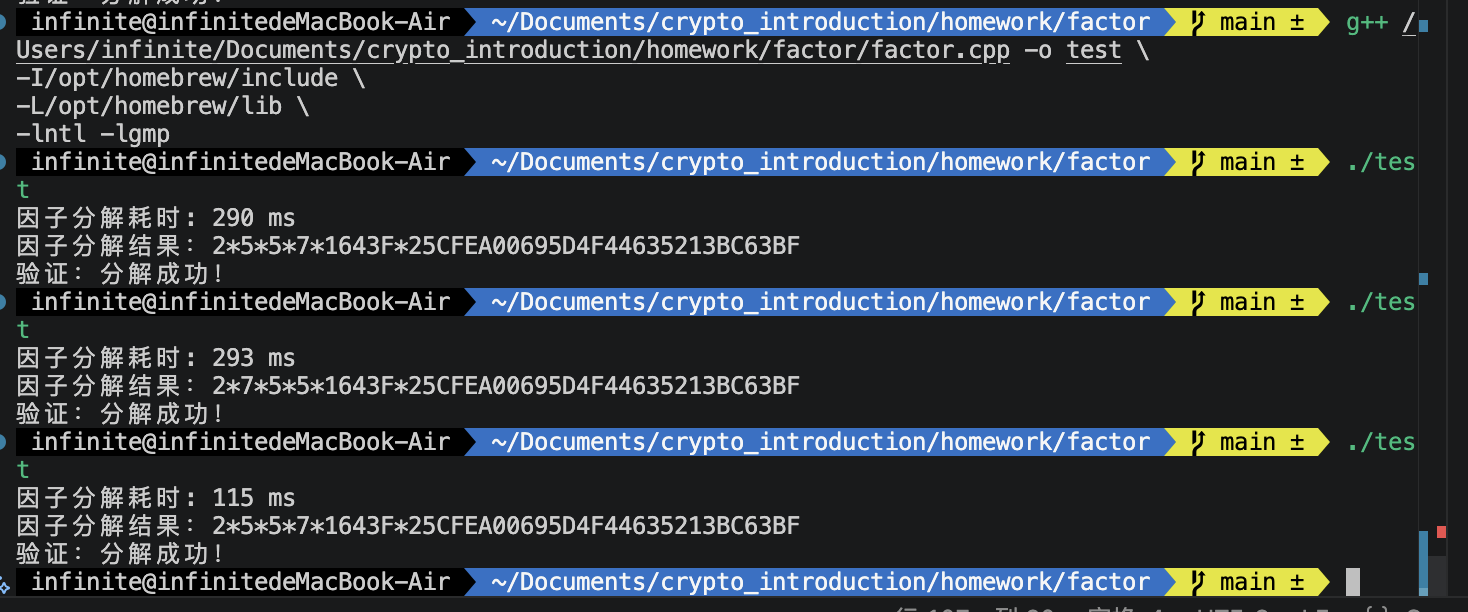
\includegraphics[width=0.8\textwidth]{result.png}
    \caption{因子分解结果}
\end{figure}
即
\[
n = 2 \times 5^2 \times 7 \times 1643F \times 25CFEA00695D4F44635213BC63BF
\]
运行三次用时$290,293,115\,\mathrm{ms}$，CPU型号为Apple M4
\end{enumerate}
\end{document}